\subsection{Experiment 6: Temperature Encoding} \label{sec:experiment-6}

\subsubsection{Objective}

When a symbol is represented as a temperature encoded vector, the symbol is represented as an array where a number of consecutive elements equal to the value of the digit being represented are set to one, the rest are set to zero. Figure \ref{fig:temperature-encoding} shows a depiction of a temperature encoded symbol of the number 5. We believe that symbols encoded using this representation can capture the quantitative and ordinal meaning of the digits and would therefore help the recurrent neural network learn an algorithm for arithmetic operations as opposed to simply learning a classifier or mapping function.

The goal of this experiment is to determine empirically whether or not models trained using the temperature encoded symbols have the ability to discover a decision function that can represent the algorithm that performs addition. We constrain the experiment to only use symbols as in Experiment 5. The models accept a sequence of operands encoded in the temperature encoding and outputs values encoded in the temperature encoding as well. The performance of the trained model is tested against both the training set as well as an unseen test set to determine if the model can generalize to unseen combinations of operands. 

\subsubsection{Method}

\begin{figure}
	\centering
	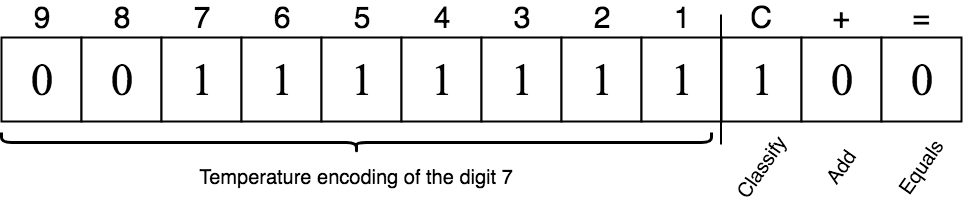
\includegraphics[max width=\textwidth]{experiment-6-input}
	\caption{An example of an input vector for the digit 7 on the first time step. The first nine features are for the temperature encoded symbol. The 10th (C) feature when set, instructs the RNN to output the class at that time step. The 11th (+) feature when set, instructs the network to output the least significant digit of the result. The 12th (=) feature when set, instructs the RNN to output the most significant digit of the result.}
	\label{fig:experiment-6-input}
\end{figure}

Three models are developed that learn to perform addition on temperature encoded symbols. Figure \ref{fig:sequential-model-temperature-symbols} shows an example of a recurrent neural network using temperature encoding to learn to do addition. The models accept a sequence of four vectors 12 elements each. Figure \ref{fig:experiment-6-input} depicts an example input. The first nine elements hold an operand represented as a symbol encoded using a temperature encoding. The 10th element indicates to the network to classify the input, meaning that if it is set to one, the model should output the same input digit using the same temperature encoding. The 11th element indicates the addition operator and the model should output the least significant digit of the result of the addition. Finally, the 12th element represents the equals sign, indicating to the model to output the most significant digit of the result. The output of each of the networks is a nine-element vector that represents the temperature encoding of the output. The following are the various architectures that were tried:
\begin{itemize}
	\item \textbf{Model A}: Two hidden layers, 20 units each.
	\item \textbf{Model B}: Two hidden layers, 10 units each.
	\item \textbf{Model C}: Two hidden layers, 5 units each.
\end{itemize}

\begin{figure}
	\centering
	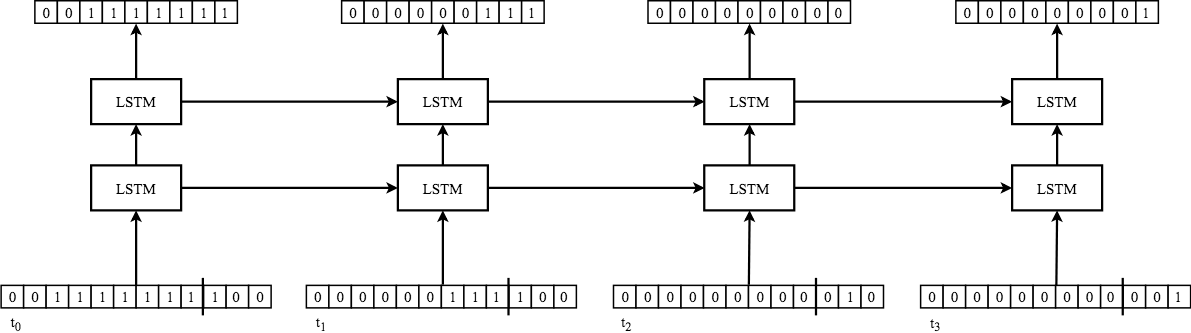
\includegraphics[max width=\textwidth]{sequential-model-temperature-symbols}
	\caption{A sequential model constrained to use symbols only. However, the symbols are encoded using temperature encoding. In this case the model is learning to perform 7 + 3. The output on the third time step (least significant time step) is all zeros to encode 0.}
	\label{fig:sequential-model-temperature-symbols}
\end{figure}

A similar dataset like the one used in Experiment 5 is used for this experiment. A subset of 80 combinations are selected for training from the 100 combinations of operands, making sure that each unique digit would be present at least once on either side of the addition operator. That same training set is also used for validation and as the test set of seen combinations. The remaining 20 combinations are used as the unseen combinations test set. Each model is trained and tested five times and the mean accuracy of each model is recorded when applying both the seen test set and the unseen test set on the trained model. Training is performed over 5000 epochs in batches of 10 using the Adam optimizer algorithm and the mean square error loss function with a learning rate of 0.001. 

\subsubsection{Results}

\begin{table}
	\center
	\caption{A comparison of the mean accuracy of each of the models trained using the temperature encoding when tested on the test set of \textbf{seen} combinations as well as the test set of \textbf{unseen} combinations.}
	\label{tab:experiment-7-results-table}
	\begin{tabular}{ |c|c|c| } 
		\hline
		Model & Accuracy - Seen (\%) & Accuracy - Unseen (\%)\\ 
		Model A & 100.0 & 90.0\\  
		Model B & 100.0 & 93.0\\  
		Model C & 100.0 & 86.0\\  
		\hline
	\end{tabular}
\end{table}

Table \ref{tab:experiment-7-results-table} shows the results obtained for each of the architectures trained. The table presents the mean accuracies of each architecture when tested on both the dataset of seen combinations and the dataset of unseen combinations. 

\subsubsection{Discussion}

\begin{figure}
	\centering
	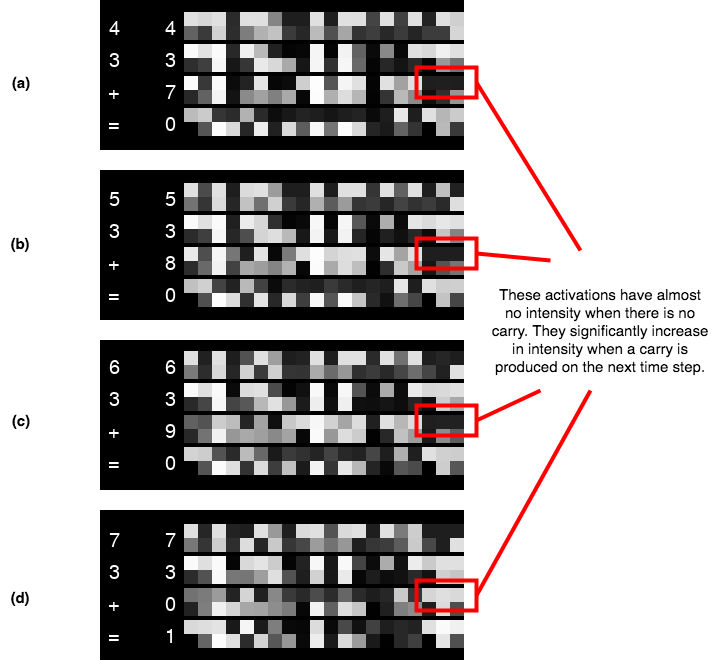
\includegraphics[max width=\textwidth]{activations-cluster-carry-temperature}
	\caption{A series of activations produced when applying examples from the unseen test set to Model A, trained using temperature encoded symbols. The activations show how the intensity in the top right region of the third time step indicates if a carry should be generated.}%
	\label{fig:activations-cluster-carry-temperature}%
\end{figure}

We can see from the results in Table \ref{tab:experiment-7-results-table} that the models perform perfectly on the training combinations and are also relatively successful at generalizing to the unseen combinations. This shows that the temperature encoded symbols that take into account the ordinal nature of the digits allow the recurrent neural networks to capture an algorithm that performs addition.

\begin{figure}%
	\centering
	\subfloat[Activations for 4 + 3]{{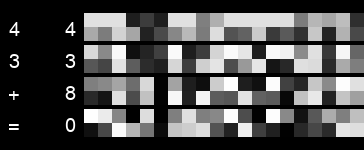
\includegraphics[width=0.5\textwidth]{activations-cluster-no-carry-4-3} }}%
	\subfloat[Activations for 5 + 3]{{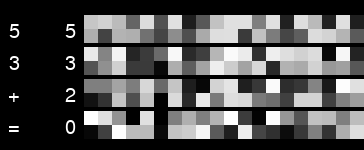
\includegraphics[width=0.5\textwidth]{activations-cluster-no-carry-5-3} }}%
	
	\subfloat[Activations for 6 + 3]{{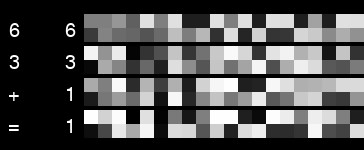
\includegraphics[width=0.5\textwidth]{activations-cluster-no-carry-6-3} }}%
	\subfloat[Activations for 7 + 3]{{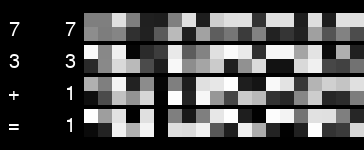
\includegraphics[width=0.5\textwidth]{activations-cluster-no-carry-7-3} }}%
	\caption{A series of activations produced when applying examples from the unseen test set to Model D of Experiment 5, trained using one-hot vector symbols. No discernible patterns are visible.}%
	\label{fig:activations-cluster-no-carry}%
\end{figure}

To further verify this conclusion, we generated activations clusters for a series of combinations from the unseen test set using Model A. Figure \ref{fig:activations-cluster-carry-temperature} shows the activations produced. In addition, Model D from the previous experiment (Experiment 5 in Section \ref{sec:experiment-5}) was retrained making sure that the same combinations shown in Figure \ref{fig:activations-cluster-carry-temperature} are part of the unseen test set. The activations for that model are shown in Figure \ref{fig:activations-cluster-no-carry}. The activations generated by the model trained using the temperature encoded symbols exhibit consistency among the same operands. Also, the region indicated at the top right end of the third time step shows a clearer carry forward signal than the one seen in Figure \ref{fig:activations-cluster-carry-temperature}. When we contrast these activations with the ones shown in Figure \ref{fig:activations-cluster-no-carry} we see that the model trained with one-hot vector symbols do not depict these clear patterns when applied to the unseen test set.

Experiments 5 and 6 show that symbols improve the accuracy of neural networks by aiding the learning algorithm in discovering a representation that capture some aspects of the algorithm that performs the operation. Temperature encoded symbols allow the models to capture more aspects. Specifically, the quantity and ordinal relationship of the operands. This results in better generalization. In the next and final experiment, we replicate Experiment 4 but this time, instead of using the one-hot vectors we use temperature encoded symbols.